\documentclass[]{article}
\usepackage{lmodern}
\usepackage{amssymb,amsmath}
\usepackage{ifxetex,ifluatex}
\usepackage{fixltx2e} % provides \textsubscript
\ifnum 0\ifxetex 1\fi\ifluatex 1\fi=0 % if pdftex
  \usepackage[T1]{fontenc}
  \usepackage[utf8]{inputenc}
\else % if luatex or xelatex
  \ifxetex
    \usepackage{mathspec}
  \else
    \usepackage{fontspec}
  \fi
  \defaultfontfeatures{Ligatures=TeX,Scale=MatchLowercase}
  \newcommand{\euro}{€}
\fi
% use upquote if available, for straight quotes in verbatim environments
\IfFileExists{upquote.sty}{\usepackage{upquote}}{}
% use microtype if available
\IfFileExists{microtype.sty}{%
\usepackage{microtype}
\UseMicrotypeSet[protrusion]{basicmath} % disable protrusion for tt fonts
}{}
\usepackage[margin=1in]{geometry}
\usepackage{hyperref}
\PassOptionsToPackage{usenames,dvipsnames}{color} % color is loaded by hyperref
\hypersetup{unicode=true,
            pdftitle={tseries},
            pdfauthor={Jose Luis Contreras Santos and Antonio Javier González Ferrer},
            pdfborder={0 0 0},
            breaklinks=true}
\urlstyle{same}  % don't use monospace font for urls
\usepackage{color}
\usepackage{fancyvrb}
\newcommand{\VerbBar}{|}
\newcommand{\VERB}{\Verb[commandchars=\\\{\}]}
\DefineVerbatimEnvironment{Highlighting}{Verbatim}{commandchars=\\\{\}}
% Add ',fontsize=\small' for more characters per line
\usepackage{framed}
\definecolor{shadecolor}{RGB}{248,248,248}
\newenvironment{Shaded}{\begin{snugshade}}{\end{snugshade}}
\newcommand{\KeywordTok}[1]{\textcolor[rgb]{0.13,0.29,0.53}{\textbf{{#1}}}}
\newcommand{\DataTypeTok}[1]{\textcolor[rgb]{0.13,0.29,0.53}{{#1}}}
\newcommand{\DecValTok}[1]{\textcolor[rgb]{0.00,0.00,0.81}{{#1}}}
\newcommand{\BaseNTok}[1]{\textcolor[rgb]{0.00,0.00,0.81}{{#1}}}
\newcommand{\FloatTok}[1]{\textcolor[rgb]{0.00,0.00,0.81}{{#1}}}
\newcommand{\ConstantTok}[1]{\textcolor[rgb]{0.00,0.00,0.00}{{#1}}}
\newcommand{\CharTok}[1]{\textcolor[rgb]{0.31,0.60,0.02}{{#1}}}
\newcommand{\SpecialCharTok}[1]{\textcolor[rgb]{0.00,0.00,0.00}{{#1}}}
\newcommand{\StringTok}[1]{\textcolor[rgb]{0.31,0.60,0.02}{{#1}}}
\newcommand{\VerbatimStringTok}[1]{\textcolor[rgb]{0.31,0.60,0.02}{{#1}}}
\newcommand{\SpecialStringTok}[1]{\textcolor[rgb]{0.31,0.60,0.02}{{#1}}}
\newcommand{\ImportTok}[1]{{#1}}
\newcommand{\CommentTok}[1]{\textcolor[rgb]{0.56,0.35,0.01}{\textit{{#1}}}}
\newcommand{\DocumentationTok}[1]{\textcolor[rgb]{0.56,0.35,0.01}{\textbf{\textit{{#1}}}}}
\newcommand{\AnnotationTok}[1]{\textcolor[rgb]{0.56,0.35,0.01}{\textbf{\textit{{#1}}}}}
\newcommand{\CommentVarTok}[1]{\textcolor[rgb]{0.56,0.35,0.01}{\textbf{\textit{{#1}}}}}
\newcommand{\OtherTok}[1]{\textcolor[rgb]{0.56,0.35,0.01}{{#1}}}
\newcommand{\FunctionTok}[1]{\textcolor[rgb]{0.00,0.00,0.00}{{#1}}}
\newcommand{\VariableTok}[1]{\textcolor[rgb]{0.00,0.00,0.00}{{#1}}}
\newcommand{\ControlFlowTok}[1]{\textcolor[rgb]{0.13,0.29,0.53}{\textbf{{#1}}}}
\newcommand{\OperatorTok}[1]{\textcolor[rgb]{0.81,0.36,0.00}{\textbf{{#1}}}}
\newcommand{\BuiltInTok}[1]{{#1}}
\newcommand{\ExtensionTok}[1]{{#1}}
\newcommand{\PreprocessorTok}[1]{\textcolor[rgb]{0.56,0.35,0.01}{\textit{{#1}}}}
\newcommand{\AttributeTok}[1]{\textcolor[rgb]{0.77,0.63,0.00}{{#1}}}
\newcommand{\RegionMarkerTok}[1]{{#1}}
\newcommand{\InformationTok}[1]{\textcolor[rgb]{0.56,0.35,0.01}{\textbf{\textit{{#1}}}}}
\newcommand{\WarningTok}[1]{\textcolor[rgb]{0.56,0.35,0.01}{\textbf{\textit{{#1}}}}}
\newcommand{\AlertTok}[1]{\textcolor[rgb]{0.94,0.16,0.16}{{#1}}}
\newcommand{\ErrorTok}[1]{\textcolor[rgb]{0.64,0.00,0.00}{\textbf{{#1}}}}
\newcommand{\NormalTok}[1]{{#1}}
\usepackage{graphicx,grffile}
\makeatletter
\def\maxwidth{\ifdim\Gin@nat@width>\linewidth\linewidth\else\Gin@nat@width\fi}
\def\maxheight{\ifdim\Gin@nat@height>\textheight\textheight\else\Gin@nat@height\fi}
\makeatother
% Scale images if necessary, so that they will not overflow the page
% margins by default, and it is still possible to overwrite the defaults
% using explicit options in \includegraphics[width, height, ...]{}
\setkeys{Gin}{width=\maxwidth,height=\maxheight,keepaspectratio}
\setlength{\parindent}{0pt}
\setlength{\parskip}{6pt plus 2pt minus 1pt}
\setlength{\emergencystretch}{3em}  % prevent overfull lines
\providecommand{\tightlist}{%
  \setlength{\itemsep}{0pt}\setlength{\parskip}{0pt}}
\setcounter{secnumdepth}{0}

%%% Use protect on footnotes to avoid problems with footnotes in titles
\let\rmarkdownfootnote\footnote%
\def\footnote{\protect\rmarkdownfootnote}

%%% Change title format to be more compact
\usepackage{titling}

% Create subtitle command for use in maketitle
\newcommand{\subtitle}[1]{
  \posttitle{
    \begin{center}\large#1\end{center}
    }
}

\setlength{\droptitle}{-2em}
  \title{tseries}
  \pretitle{\vspace{\droptitle}\centering\huge}
  \posttitle{\par}
  \author{Jose Luis Contreras Santos and Antonio Javier González Ferrer}
  \preauthor{\centering\large\emph}
  \postauthor{\par}
  \predate{\centering\large\emph}
  \postdate{\par}
  \date{December 21st, 2016}


\usepackage{float}
\usepackage{hyperref}

% Redefines (sub)paragraphs to behave more like sections
\ifx\paragraph\undefined\else
\let\oldparagraph\paragraph
\renewcommand{\paragraph}[1]{\oldparagraph{#1}\mbox{}}
\fi
\ifx\subparagraph\undefined\else
\let\oldsubparagraph\subparagraph
\renewcommand{\subparagraph}[1]{\oldsubparagraph{#1}\mbox{}}
\fi

\begin{document}
\maketitle

\subsection{Loading the data}\label{loading-the-data}

\begin{Shaded}
\begin{Highlighting}[]
\KeywordTok{library}\NormalTok{(forecast)}
\KeywordTok{library}\NormalTok{(astsa)}
\KeywordTok{library}\NormalTok{(tseries)}
\KeywordTok{library}\NormalTok{(car)}
\KeywordTok{library}\NormalTok{(astsa)}

\NormalTok{visados.df <-}\StringTok{ }\KeywordTok{read.csv}\NormalTok{(}\StringTok{"../data/data_g2.csv"}\NormalTok{, }\DataTypeTok{header=}\NormalTok{T, }\DataTypeTok{sep=}\StringTok{","}\NormalTok{, }\DataTypeTok{stringsAsFactors =} \OtherTok{FALSE}\NormalTok{)}
\CommentTok{# Create a Time Series object, starting from 1997 and seasonal data.}
\NormalTok{visados.ts <-}\StringTok{ }\KeywordTok{ts}\NormalTok{(visados.df$Visados, }\DataTypeTok{start=}\KeywordTok{c}\NormalTok{(}\DecValTok{1997}\NormalTok{,}\DecValTok{1}\NormalTok{), }\DataTypeTok{end=}\KeywordTok{c}\NormalTok{(}\DecValTok{2013}\NormalTok{, }\DecValTok{8}\NormalTok{), }\DataTypeTok{frequency =} \DecValTok{12}\NormalTok{)}
\end{Highlighting}
\end{Shaded}

\subsection{Part 1}\label{part-1}

Jose --\textgreater{}

\subsection{Part 2}\label{part-2}

Decomposition methods describe the trend and seasonal factors in a time
series. We will use this information for understanding the data at hand
before building a more sophisticated model, for instance, an ARIMA
model.

The Multiplicative decomposition is one of the basic decomposition
methods and it is useful when the seasonal variance of the data
increases over time. As we will see in section X, such hypothesis will
be closer to the structure of the dataset than the simple Additive
decomposition. The Multiplicative decomposition method is defined as
follows:

\[x_t = T_t * S_t * I_t\]

where \(x_t\) is the time series at time \(t\), \(T_t\) is the trend,
\(S_t\) is the seasonality and \(I_t\) is the irregular part or
remainder. Essentially, the goal is to find a decomposition such that
the remainder behaves like white noise, that is to say, the remainder
acts as a stationary time series by itself.

There are different ways to model the trend and the seasonality
components. R provides the stl() function for seasonal decomposition of
time series based on LOESS, a smoothing procedure that is based on
local, weighted robust regression. The aim of this procedure is to
reduce potentially the disturbing influence of outliers. By default, the
command stl() performs an additive decomposition but it can be easily
transformed to a multiplicative decomposition taking logarithm of the
input data.

\begin{Shaded}
\begin{Highlighting}[]
\CommentTok{# Multiplicative decomposition}
\NormalTok{visados.stl <-}\StringTok{ }\KeywordTok{stl}\NormalTok{(}\KeywordTok{log}\NormalTok{(visados.ts), }\DataTypeTok{s.window=}\StringTok{"periodic"}\NormalTok{)}
\KeywordTok{plot}\NormalTok{(visados.stl)}
\end{Highlighting}
\end{Shaded}

\begin{figure}[H]

{\centering 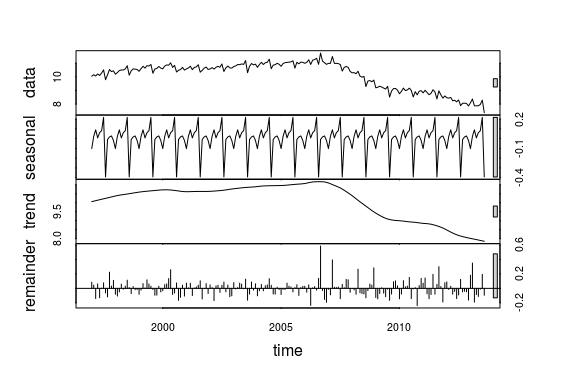
\includegraphics{tseries_files/figure-latex/decomposition-1} 

}

\caption{Pedro picapiedra}\label{fig:decomposition}
\end{figure}

The second parameter essentially controls the seasonal effects to be
estimated in as averages of de-trended values. The plot shows the
observed series, the seasonal pattern, the smoothed trend line, and the
remainder part of the series. Note that the seasonal pattern is a
regularly repeating pattern. The grey bars facilitate the interpretation
by covering the same span of the \(y\)-scale in all the charts.

Nevertheless, the remainder does not look like white noise. Looking at
the ACF plot, some significant autocorrelation coefficients can be
distinguished outside the limits. Then, there is still information left
in the remainder that should be used in computing forecasts.

\begin{Shaded}
\begin{Highlighting}[]
\CommentTok{# Extracting and ploting the remainder part.}
\NormalTok{visados.stl.remainder <-}\StringTok{ }\NormalTok{visados.stl$time.series[,}\KeywordTok{c}\NormalTok{(}\StringTok{"remainder"}\NormalTok{)]}
\KeywordTok{tsdisplay}\NormalTok{(visados.stl.remainder)}
\end{Highlighting}
\end{Shaded}

\begin{figure}[H]

{\centering 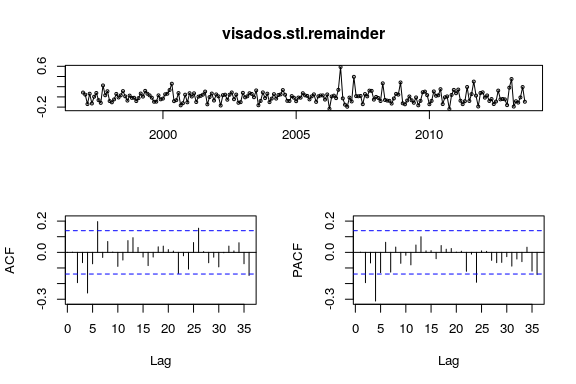
\includegraphics{tseries_files/figure-latex/remainder-1} 

}

\caption{Pedro picapiedra}\label{fig:remainder}
\end{figure}

The further assumption is checked using the Box-Pierce test for
examining the null hypothesis of independence in the remainder. The
\(p\)-value is close to 0 and hence there exist significant
autocorrelations for the first 12 lags.

\begin{Shaded}
\begin{Highlighting}[]
\CommentTok{# Box-Pierce test for independence of a time series.}
\KeywordTok{Box.test}\NormalTok{(visados.stl.remainder, }\DataTypeTok{lag=}\DecValTok{12}\NormalTok{) }
\end{Highlighting}
\end{Shaded}

\begin{verbatim}
## 
##  Box-Pierce test
## 
## data:  visados.stl.remainder
## X-squared = 35.136, df = 12, p-value = 0.0004454
\end{verbatim}

Let us forecast future values based on the last analysis of the trend
and seasonal factors.

\begin{Shaded}
\begin{Highlighting}[]
\KeywordTok{plot}\NormalTok{(}\KeywordTok{forecast}\NormalTok{(visados.stl, }\DataTypeTok{method=}\StringTok{"naive"}\NormalTok{))}
\end{Highlighting}
\end{Shaded}

\begin{figure}[H]

{\centering 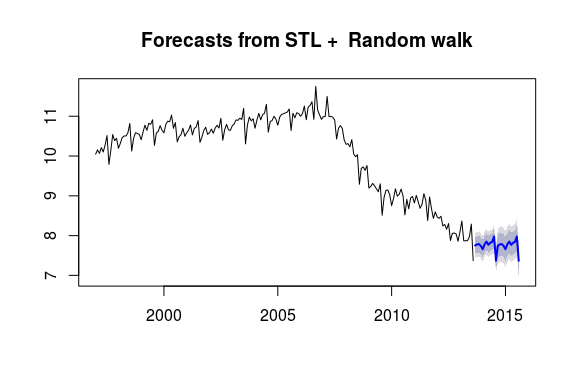
\includegraphics{tseries_files/figure-latex/forecast-1} 

}

\caption{Pedro picapiedra}\label{fig:forecast}
\end{figure}

--\textgreater{}

\subsection{Part 3}\label{part-3}

\subsubsection{Description}\label{description}

blablabla ARIMA blablbla

\subsubsection{Data transformation}\label{data-transformation}

First of all, let us decide on whether to use the original variable or
to work with the log transformation of it. The log transformation might
improve the stationary of the time series. We will select the latter
option if the amplitude of the seasional changes increases with the
overall trend, that is, if the variance is not constant across the
series. In the following figure you can observe that the shape of the
log plot is smoother and its variance is more stable than the original
variable. Therefore we will use the log of the house sales variable from
now on. Notice that the Box Cox transformation suggests to use a lambda
close to 0 too.

\begin{figure}[H]

{\centering 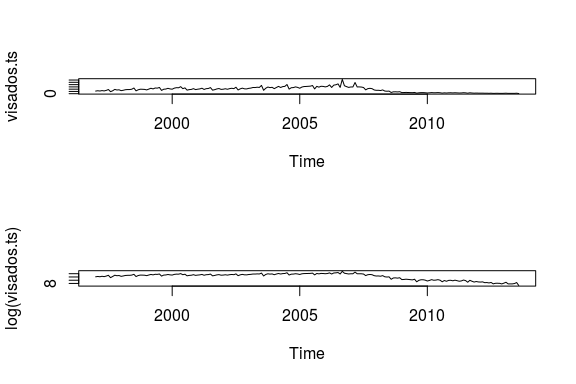
\includegraphics{tseries_files/figure-latex/variance-1} 

}

\caption{Pedro picapiedra}\label{fig:variance}
\end{figure}

\subsubsection{Seasonality}\label{seasonality}

The nature of the dataset leads us to set an anual seasonal component,
\(s=12\). Analyzing the periodogram of Figure \ref{fig:periodogram}, we
can clearly observe a high peak at point 0 of the \(x\)-axis. This peak
is related to a long repeated cycle over the time, in our case, a
12-monthly seasonality. On the other hand, the seasonplot() and
monthplot() functions might help us identifying this seasionality.
Firstly, the season plot shows how the ups and downs are similar over
the years. Secondly, the month plot reveals a strong seasonality pattern
in August, where the sales decay. This drop should be adjusted into the
model if we would like to see whether there is a real trend if the house
sales go down in August.

\begin{figure}[H]
    \centering
    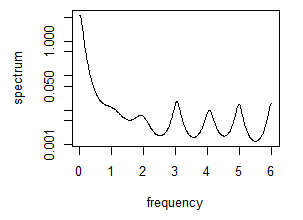
\includegraphics[width=4in]{figures/periodogram.png} 
    \caption{Periodogram of log(visados.ts)}
    \label{fig:periodogram}
\end{figure}

\begin{Shaded}
\begin{Highlighting}[]
\KeywordTok{par}\NormalTok{(}\DataTypeTok{mfrow=}\KeywordTok{c}\NormalTok{(}\DecValTok{1}\NormalTok{,}\DecValTok{2}\NormalTok{))}
\KeywordTok{seasonplot}\NormalTok{(}\KeywordTok{log}\NormalTok{(visados.ts))}
\KeywordTok{monthplot}\NormalTok{(}\KeywordTok{log}\NormalTok{(visados.ts))}
\end{Highlighting}
\end{Shaded}

\begin{figure}[H]

{\centering 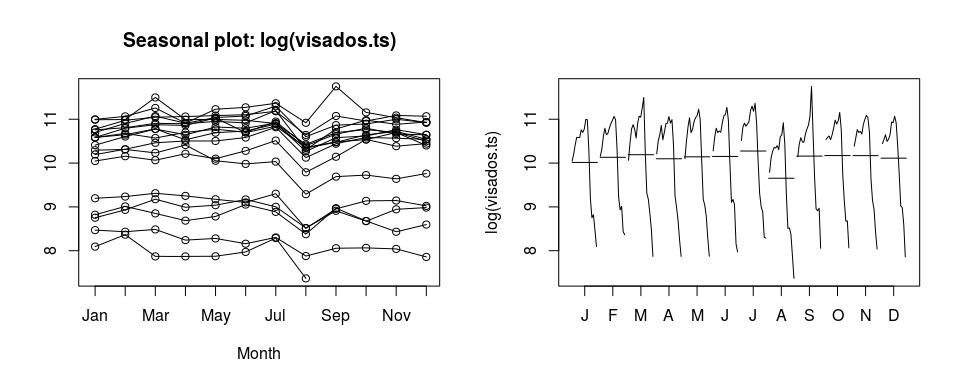
\includegraphics{tseries_files/figure-latex/seasonality-1} 

}

\caption{Pedro picapiedra}\label{fig:seasonality}
\end{figure}

\subsubsection{Differencing}\label{differencing}

The next step in fitting an ARIMA model is to detect the order of
differencing needed to make the time series stationary. We will employ
the adf.test to check stationarity and the standard deviation values to
set the stop condition (the lower, the better.)

Let us suppose that we omit the seasonality analysis from the last
section. Since the original ACF plot (Figure X) has positive
autocorrelations out to a high number of lags, we will apply one order
of diferencing.

\begin{Shaded}
\begin{Highlighting}[]
\CommentTok{# Initial standard deviation}
\KeywordTok{sd}\NormalTok{(}\KeywordTok{log}\NormalTok{(visados.ts))}
\end{Highlighting}
\end{Shaded}

\begin{verbatim}
## [1] 1.006753
\end{verbatim}

\begin{Shaded}
\begin{Highlighting}[]
\CommentTok{# tsdisplay(log(visados.ts)) #this plot should already be in the report.}

\CommentTok{# One order of differencing.}
\KeywordTok{sd}\NormalTok{(}\KeywordTok{diff}\NormalTok{(}\KeywordTok{log}\NormalTok{(visados.ts)))}
\end{Highlighting}
\end{Shaded}

\begin{verbatim}
## [1] 0.2719039
\end{verbatim}

\begin{Shaded}
\begin{Highlighting}[]
\KeywordTok{adf.test}\NormalTok{(}\KeywordTok{diff}\NormalTok{(}\KeywordTok{log}\NormalTok{(visados.ts)))}
\end{Highlighting}
\end{Shaded}

\begin{verbatim}
## Warning in adf.test(diff(log(visados.ts))): p-value smaller than printed p-
## value
\end{verbatim}

\begin{verbatim}
## 
##  Augmented Dickey-Fuller Test
## 
## data:  diff(log(visados.ts))
## Dickey-Fuller = -7.5577, Lag order = 5, p-value = 0.01
## alternative hypothesis: stationary
\end{verbatim}

\begin{Shaded}
\begin{Highlighting}[]
\KeywordTok{tsdisplay}\NormalTok{(}\KeywordTok{diff}\NormalTok{(}\KeywordTok{log}\NormalTok{(visados.ts)))}
\end{Highlighting}
\end{Shaded}

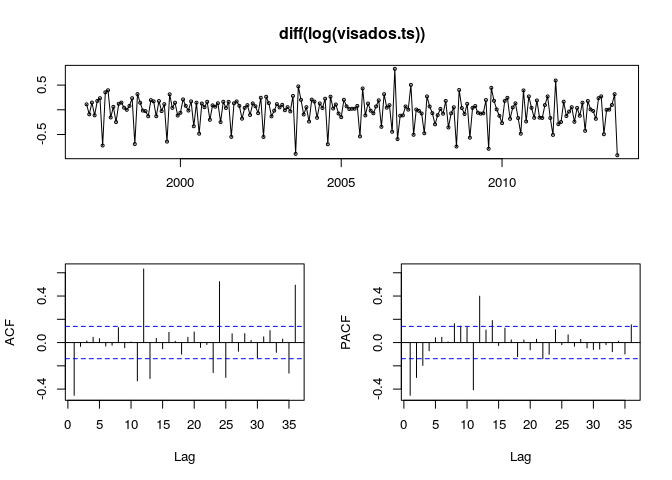
\includegraphics{tseries_files/figure-latex/first_difference-1.pdf}

We achieve stationarity due to we have evidence to reject the null
hypothesis in favor of the alternative hypothesis of stationarity in the
Augmented Dicket-Fuller test. However, notice the high peaks of
autocorrelations in the lags 12, 24 and 36. This is a clear evidence of
monthly seasonality. Therefore, we omit this first step and we apply
directly a first seasonal difference in order to see if the time series
is described by a seasonal random walk.

\begin{Shaded}
\begin{Highlighting}[]
\CommentTok{# One order of seasonal differencing.}
\KeywordTok{sd}\NormalTok{(}\KeywordTok{diff}\NormalTok{(}\KeywordTok{log}\NormalTok{(visados.ts), }\DecValTok{12}\NormalTok{))}
\end{Highlighting}
\end{Shaded}

\begin{verbatim}
## [1] 0.39003
\end{verbatim}

\begin{Shaded}
\begin{Highlighting}[]
\CommentTok{# Checking stationarity}
\KeywordTok{adf.test}\NormalTok{(}\KeywordTok{diff}\NormalTok{(}\KeywordTok{log}\NormalTok{(visados.ts), }\DecValTok{12}\NormalTok{))}
\end{Highlighting}
\end{Shaded}

\begin{verbatim}
## 
##  Augmented Dickey-Fuller Test
## 
## data:  diff(log(visados.ts), 12)
## Dickey-Fuller = -1.8166, Lag order = 5, p-value = 0.6529
## alternative hypothesis: stationary
\end{verbatim}

\begin{Shaded}
\begin{Highlighting}[]
\KeywordTok{tsdisplay}\NormalTok{(}\KeywordTok{diff}\NormalTok{(}\KeywordTok{log}\NormalTok{(visados.ts), }\DecValTok{12}\NormalTok{))}
\end{Highlighting}
\end{Shaded}

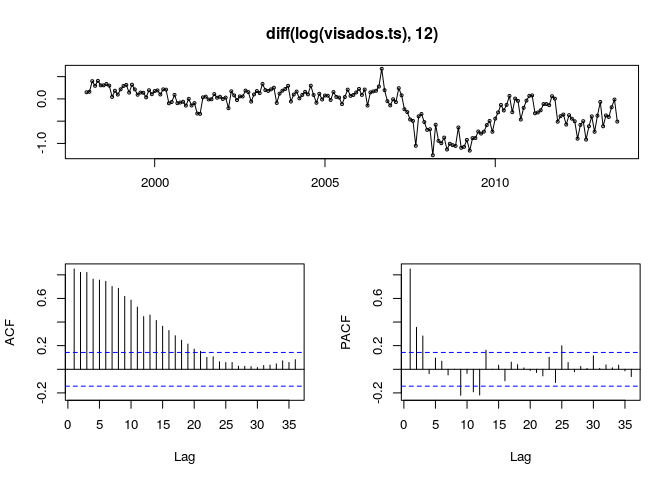
\includegraphics{tseries_files/figure-latex/first_seasonal_difference-1.pdf}
A seasonal random walk is defined as \(\hat{Y}_t = Y_{t-12} + \mu\),
where \(\mu\) is the average annnual trend. In this case, there are not
evidence to reject the null hypothesis in the adf.test() and the ACF
plot still has many positive autocorrelations. As we have already seen,
this is an evidence to apply one order of non-seasonal difference.

\begin{Shaded}
\begin{Highlighting}[]
\CommentTok{# One order of non seasonal differencing and one order of seasonal differencing.}
\KeywordTok{sd}\NormalTok{(}\KeywordTok{diff}\NormalTok{(}\KeywordTok{diff}\NormalTok{(}\KeywordTok{log}\NormalTok{(visados.ts), }\DecValTok{12}\NormalTok{)))}
\end{Highlighting}
\end{Shaded}

\begin{verbatim}
## [1] 0.2116118
\end{verbatim}

\begin{Shaded}
\begin{Highlighting}[]
\KeywordTok{adf.test}\NormalTok{(}\KeywordTok{diff}\NormalTok{(}\KeywordTok{diff}\NormalTok{(}\KeywordTok{log}\NormalTok{(visados.ts), }\DecValTok{12}\NormalTok{)))}
\end{Highlighting}
\end{Shaded}

\begin{verbatim}
## Warning in adf.test(diff(diff(log(visados.ts), 12))): p-value smaller than
## printed p-value
\end{verbatim}

\begin{verbatim}
## 
##  Augmented Dickey-Fuller Test
## 
## data:  diff(diff(log(visados.ts), 12))
## Dickey-Fuller = -6.8037, Lag order = 5, p-value = 0.01
## alternative hypothesis: stationary
\end{verbatim}

\begin{Shaded}
\begin{Highlighting}[]
\KeywordTok{tsdisplay}\NormalTok{(}\KeywordTok{diff}\NormalTok{(}\KeywordTok{diff}\NormalTok{(}\KeywordTok{log}\NormalTok{(visados.ts), }\DecValTok{12}\NormalTok{)))}
\end{Highlighting}
\end{Shaded}

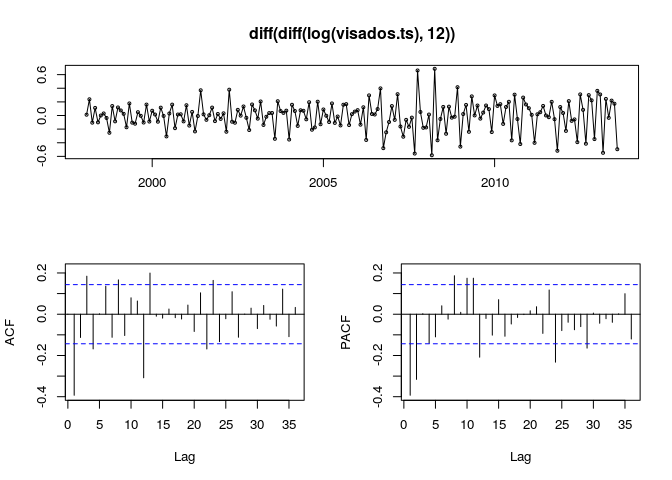
\includegraphics{tseries_files/figure-latex/seasonal_and_non_seasonal-1.pdf}
We obtain stationarity again, with a lower standard deviation and the
peaks in the lags 12 and 24 are considerably smaller. The times series
is now modeled as a seasonal random trend. Comparing this model with the
seasonal random walk, they both predict that next year`s seasonal cycle
will have the same pattern. In contrast, the seasonal random trend
considers that the future trend will be equal to the
\(\underline{\text{most recent}}\) year-to-year trend, instead of the
\(\underline{\text{average}}\) year-to-year trend (\(\mu\) in the
model). The seasonal random trend is defined as
\(\hat{Y}_t = Y_{t-12} + Y_{t-1} - Y{t-13}\), which is equivalent to an
\(ARIMA(0,1,0)(0,1,0)_{12}\) model.

To conclude, we stop here since another order of differencing does not
improve the standard deviation. On the other hand, notice

\begin{Shaded}
\begin{Highlighting}[]
\KeywordTok{sd}\NormalTok{(}\KeywordTok{diff}\NormalTok{(}\KeywordTok{diff}\NormalTok{(}\KeywordTok{diff}\NormalTok{(}\KeywordTok{log}\NormalTok{(visados.ts), }\DecValTok{12}\NormalTok{))))}
\end{Highlighting}
\end{Shaded}

\begin{verbatim}
## [1] 0.3522928
\end{verbatim}

Let us study what values of differencing the functions ndiffs and
ndsdiff suggest. These results should be taken into account with a grain
of salt, and just use them to support our analysis.

\begin{Shaded}
\begin{Highlighting}[]
\KeywordTok{ndiffs}\NormalTok{(}\KeywordTok{log}\NormalTok{(visados.ts), }\DataTypeTok{test=}\StringTok{"kpss"}\NormalTok{)}
\end{Highlighting}
\end{Shaded}

\begin{verbatim}
## [1] 2
\end{verbatim}

\begin{Shaded}
\begin{Highlighting}[]
\KeywordTok{ndiffs}\NormalTok{(}\KeywordTok{log}\NormalTok{(visados.ts), }\DataTypeTok{test=}\StringTok{"adf"}\NormalTok{)}
\end{Highlighting}
\end{Shaded}

\begin{verbatim}
## [1] 1
\end{verbatim}

\begin{Shaded}
\begin{Highlighting}[]
\KeywordTok{nsdiffs}\NormalTok{(}\KeywordTok{log}\NormalTok{(visados.ts), }\DataTypeTok{m=}\DecValTok{12}\NormalTok{)}
\end{Highlighting}
\end{Shaded}

\begin{verbatim}
## [1] 0
\end{verbatim}

Surprisingly, depending on the test we use to estimate the number of
differences required to make the time series stationary, we obtain a
different value. This extra differencing order is a particular case
where the KPPS test detects that the first order difference of the time
series is still not stationary but trend-stationary, and another order
of differencing is needed. In contrast, the ADF test just rejects the
null hypothesis of present of a unit root. On the other hand, nsdiffs
indicates the need of non order of seasonal differencing.

\end{document}
